\documentclass{sigchi}


%% EXAMPLE BEGIN -- HOW TO OVERRIDE THE DEFAULT COPYRIGHT STRIP -- (July 22, 2013 - Paul Baumann)
% \toappear{Permission to make digital or hard copies of all or part of this work for personal or classroom use is      granted without fee provided that copies are not made or distributed for profit or commercial advantage and that copies bear this notice and the full citation on the first page. Copyrights for components of this work owned by others than ACM must be honored. Abstracting with credit is permitted. To copy otherwise, or republish, to post on servers or to redistribute to lists, requires prior specific permission and/or a fee. Request permissions from permissions@acm.org. \\
% {\emph{CHI'14}}, April 26--May 1, 2014, Toronto, Canada. \\
% Copyright \copyright~2014 ACM ISBN/14/04...\$15.00. \\
% DOI string from ACM form confirmation}
%% EXAMPLE END -- HOW TO OVERRIDE THE DEFAULT COPYRIGHT STRIP -- (July 22, 2013 - Paul Baumann)


% Arabic page numbers for submission.  Remove this line to eliminate
% page numbers for the camera ready copy 

\pagenumbering{arabic}

% Load basic packages
\usepackage{balance}  % to better equalize the last page
\usepackage{graphics} % for EPS, load graphicx instead 
%\usepackage[T1]{fontenc}
\usepackage{txfonts}
\usepackage{times}    % comment if you want LaTeX's default font
\usepackage[pdftex]{hyperref}
% \usepackage{url}      % llt: nicely formatted URLs
\usepackage{color}
\usepackage{textcomp}
\usepackage{booktabs}
\usepackage{ccicons}
\usepackage{todonotes}

\usepackage{subcaption}


% llt: Define a global style for URLs, rather that the default one
\makeatletter
\def\url@leostyle{%
  \@ifundefined{selectfont}{\def\UrlFont{\sf}}{\def\UrlFont{\small\bf\ttfamily}}}
\makeatother
\urlstyle{leo}

% To make various LaTeX processors do the right thing with page size.
\def\pprw{8.5in}
\def\pprh{11in}
\special{papersize=\pprw,\pprh}
\setlength{\paperwidth}{\pprw}
\setlength{\paperheight}{\pprh}
\setlength{\pdfpagewidth}{\pprw}
\setlength{\pdfpageheight}{\pprh}

% Make sure hyperref comes last of your loaded packages, to give it a
% fighting chance of not being over-written, since its job is to
% redefine many LaTeX commands.
\definecolor{linkColor}{RGB}{6,125,233}
\hypersetup{%
  pdftitle={SIGCHI Conference Proceedings Format},
  pdfauthor={LaTeX},
  pdfkeywords={SIGCHI, proceedings, archival format},
  bookmarksnumbered,
  pdfstartview={FitH},
  colorlinks,
  citecolor=black,
  filecolor=black,
  linkcolor=black,
  urlcolor=linkColor,
  breaklinks=true,
}

% create a shortcut to typeset table headings
% \newcommand\tabhead[1]{\small\textbf{#1}}

% End of preamble. Here it comes the document.
  \begin{document}

%\title{Quantitative Evaluation of Touch-Screen Group Musical Performance with
 % Transition Matrix Measures}
%\title{Mining interaction log data in long-term practice-led research}
 
\title{Mining Interaction Log Data in a Creative Arts Practice using Macro Gestures and Transition Matrices}


%in a Creative Arts Practice}

\numberofauthors{3}
\author{%
  \alignauthor{1st Author Name\\
    \affaddr{Affiliation}\\
    \affaddr{City, Country}\\
    \email{e-mail address}}\\
  \alignauthor{2nd Author Name\\
    \affaddr{Affiliation}\\
    \affaddr{City, Country}\\
    \email{e-mail address}}\\
  \alignauthor{3rd Author Name\\
    \affaddr{Affiliation}\\
    \affaddr{City, Country}\\
    \email{e-mail address}}\\
}

\maketitle

\begin{abstract}

%consider the following? .............


%   %Digital arts practices can allow for the archival of interaction
% log data. Such log data can capture and preserve performances of
% new-media artists and musicians and %and can facilitate post-hoc data
% processing and data mining.
  
  In this note we describe the analysis of a data archive for an iPad
  musical-ensemble performance practice where transition matrix
  measures are able to distinguish between sessions of different
  contexts, and the internal structure of these sessions. The archive
  includes 95 touch data logs of ensemble touch-screen interactions in
  concerts, rehearslas and formal HCI studies of groups of musicians
  over more than two years.


  % At the lowest level, data for each musician in a particular
  % performance was archived as Apple iOS callback methods for
  % touching and swiping.

  The data analysis has been undertaken by first classifying
  these data into higher level gesture types and then describing the
  transitions between these gestures for each artist as a function of
  time. We find that a transition-matrix measure, which we call
  ``flux'', can be used to distinguish different performance types and
  contexts, as well as different phases (beginning, middle and end) of
  all of the performances in our corpus.

\end{abstract}

\keywords{  Creativity Support Tools;
  Agent; 
  Design;
  Methodology}

\category{H.5.5.}{Information Interfaces and Presentation
  (e.g. HCI)}{Sound and Music Computing}{ Systems} 

% \category{See
%   \url{http://acm.org/about/class/1998/} for the full list of ACM
%   classifiers. This section is required.}{}{}

%\section{General comments}

% \begin{itemize}
% \item we should be clear (and careful) where we're talking about
%   groups TMs, and where we're talking about individual performers
% \item what's the terminology we're using for a ``performance''? Is it
%   ``performance'', or is that too music-specific? ``Session''?
%   Alternatives are ``activity'', or ``interaction'', but they're so
%   general\ldots This decision has implications for our other
%   terminology: participant vs performer vs musician, etc.
% \item Title: maybe ``Traces through time: making sense of longitudinal
%   open-ended interaction data'' or some such? I think that's our big
%   contribution: it takes the in-the-wild, practitioner-driven research
%   program stuff and tries to make some quantitative sense out of it
%   post-hoc.
% \end{itemize}

\section{Introduction}

\begin{figure*}
  \centering
  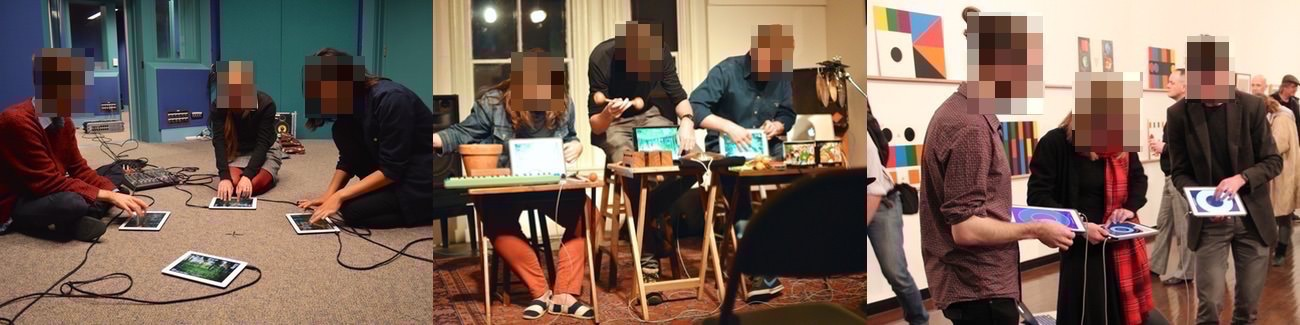
\includegraphics[width=\linewidth]{figures/three-performance-contexts}
  \caption{Collaborative musical interaction with our touch-screen
    interfaces in three different contexts: (left to right) rehearsal
    in a studio,
    performance in front of an audience, and demonstration at a
    research poster session. All of these session were improvised,
    and in the performance session, the musicians used percussion
    instruments as well as iPads.
    \label{fig:three-performance-contexts}}
\end{figure*}


Modern computing devices and interfaces continue to open up open-ended
creative opportunities for new artistic experiences. Understanding and
evaluating interfaces in these contexts presents many
challenges~\cite{Resnick:2005yu,Shneiderman:2007qv}.

In the context of live performance, interface evaluation, using, for
example, post-performance questionnaires, can omit consideration of
the dynamic needs of artists in the moment of the performance and in
the wild of the performance context. 

In contrast to traditional art forms, logged interaction data from
interaction with a computer-based artistic interface can provide an
enduring record of that performance for post-hoc quantitative
investigation as well as for curation and
preservation~\cite{England:2014ys}. 

Over time, the accumulation of
interaction log data might allow data-mining techniques to be deployed
to potentially describe universal features of such interaction.

% Additionally, a wider dissemination of such log data will better
% support the replication of findings in HCI
% research~\cite{Wilson:2011ve}

It is a feature of creative expression in the arts that highly skilled
practitioners exploit simple tools to produce works of beauty whether
it be static paintings or dynamic performance. 

In previous work~\cite{Martin:2014cr} researchers have shown that
trained percussionists can exploit a very simple iPad interface to
discover new categories of musical gestures.

In that paper, iPad apps
were studied where tapping was mapped to produce produced short
sounds, while swiping produced long sounds with the volume
proportional to the velocity of the moving touch point. 

It turned out that trained percussionists working together in an
ensemble were able to discover and repeatedly make use of five macro
gestures made up of taps and swipes: fast taps, slow taps, random
taps, short swipes and swirls. This process of discovery of
interesting musical gestures from a simple interface is analogous to
what percussionists do with acoustic instruments -- drums and bowls
and bells are often tapped, stroked and hit in novel ways to
communicate meaning and emotion through music~\cite{Schick:2006fk}.



In this note we describe a log data archive that has been accumulated
to support a long-term practice-led research program into simple iPad
interfaces for group music-making similar to those described in Martin
et al~\cite{Martin:2014cr}. Over a period of more than two years
(April 2013--June 2015), we collected data from group music-making
sessions where the participants used custom-built, touch-screen apps
on Apple iPad devices. 
Although several different apps have been
included in our corpus, they all shared the simple mode of interaction
where the majority of the screen could be used for free-form touch
interactions; tapping produced short sounds, while swiping or swirling
produced long sounds with the volume proportional to the velocity of
the moving touch point. Apart from this commonality, our apps featured
different palettes of available sounds and modes of synthesis,
different arrangements of sounds on the iPad screens, different kinds
of visual display and feedback, different kinds of networked
interactions (between the iPads in an ensemble and with a central
server), as well as a variety of special features for each app.

In all of our data-collection sessions, every touch
interaction---every touch down, dragging movement and touch up---was
time-stamped and logged to disk for later analysis. These sessions
included rehearsals without an audience as well as live performances
at art festivals and other events. They also included two
formally-structured HCI experiments in order to understand and iterate
on the system and interface design. Some of the performances were
iPad-only and others used iPads together with other acoustic
percussion instruments. Although the majority of the sessions were
free-form improvisations, a number of rehearsals and performances
involved composed pieces where the musicians read and interpreted
percussion notation as they used the apps. Representative photographs
of some of these session contexts (rehearsal, performance including
other acoustic instruments and demonstrations) are are shown
Figure~\ref{fig:three-performance-contexts}) and other descriptive
statistics about the sessions are shown in Table \ref{corpus-table}.
In our corpus, the median length of sessions is 7m29s and the median
number of participants per ensemble is four; . Metadata is included
together with the interaction data for each session to record the
\emph{context} (performance, rehearsal, study), session \emph{type}
(improvisation or composition), and \emph{instrumentation}
(iPads-only, or iPads with acoustic percussion). The distribution of
recorded sessions by context and type is shown in Figure
\ref{fig:count-data}.


% TODO fix this table to remove descriptive data about the
% demonstration sessions.
\begin{table}
\centering
\begin{tabular}{l|llll}
\hline
            & Total & Min  & Median   & Max     \\ 
\hline
N           & 150       &         &        &  \\
%Record size & 306MB     &         &        &   \\
Length      & 20H34M22S & 1M0S    & 7M29S  & 26M0S\\
Participants& 524       & 1       & 4      & 9    \\
Flux        &           & 0.02239 & 0.1445 & 0.3246\\
%Entropy     &           &  &  & \\          
\hline
\end{tabular}
\caption{
  Representative data about the corpus of musical touch-screen
  interaction sessions used in this study. These sessions were
  rehearsals, performances, studies, and demonstration sessions and 
  participants improvised or performed compositions. Each record
  consisted of touch-data recorded in CSV format and was later analysed
  with a gestural classification system. Some participants were
  present in multiple sessions, however this data was not tracked in
  the corpus.\label{corpus-table}}
\end{table}


\section{Macro Gestures, Transition Matrices and Matrix Measures}

A useful way of modelling user interfaces is to consider their
configurations as state vectors and to deploy the methods of matrix
algebra to describe transitions between these states during an
interaction sequence~\cite{Thimbleby:2001kq, Thimbleby:2004fj}.
An opposite approach is to record users' interactions with an
interface, manually coding interaction states. 
This method has been applied to usability analysis of resource
planning software for security applications~\cite{Kannampallil:2007fp}
where the transition probability matrix of these state sequences
was used to draw conclusions about the nature of this interactions.
In the creative arts, editing commands at a computer interface for the
``live coding'' of computer music has also been coded as states and
analysed using transition matrices~\cite{Swift:2014tya}, in both the
textual and musical dimensions, in order to arrive at conclusions
regarding artistic style.

In our corpus of iPad musical performances, rehearsals and studies, we
have used the continuous touch-screen gestures identified by Martin et
al~\cite{Martin:2014cr} as a basis for a musical state-space.
Each performer in each musical piece can then be thought of as
producing a ``score'' of state transitions and an overall transition
matrix for the entire ensemble can be derived by averaging the
individual transition matrices.

Suppose that each participant's activity in a collaborative
interaction can at any given time be classified as belonging to one of
$m$ distinct \emph{states}. Over the course of the activity, each
participant $X$ generates a length $N$ sequence of these interaction
states
\begin{equation}
 X_n \hskip 2em n = 1, \ldots, N
\end{equation}
which can be thought of as Markov process. If there is an
(automated) classification process for extracting each participant's
state sequence from (or during) their interaction data, then we can
estimate the $m \times m$ transition matrix $P$ which characterises
this process by simply counting the number of times state $j$ follows
state $i$
\begin{equation}
  p_{ij} = \frac{N_{ij}}{\sum_i \sum_j N_{ij}}
\end{equation}
The transition activity of the whole ensemble can be calculated by
averaging the TM for each performer. The matrix can be normalised so
that the sum of all elements is equal to one.

Previous work~\cite{Martin:2015jk} showed that the raw touch data
obtained from interaction with simple iPad interfaces similar to ours
could be segmented using a Random Forest\cite{Breiman:2001kx}
classifier\footnote{The classifier used was from Python's Scikit-learn
  package\cite{scikit-learn}.}. The classifier was applied to 5-second
windows of the touch-data to provide a chain of gesture-states for
each participant in each session. These chains can be used to create
$9 \times 9$ (the classifier recognises 9~distinct gestures)
transition matrices for individual performers and the whole ensemble
in each session.

\section{Quantitative transition matrix statistics}
\label{sec:underst-impr-group}

While the interaction sessions recorded in our corpus were performed
by many different participants with varying experience levels, in
different contexts and on different instrumental setups, the common
interface and method of recording the data allows all the sessions to
be transformed into gesture sequences. These transition matrices have
been used as a visualisation technique to reveal qualitative
differences in structure in improvisational
music-making\cite{Swift:2014tya}. In this paper, however, we wish to
extract quantitative statistics from these TMs for comparing and
tracking different sessions over time.

To do this we calculate two high-level quantities from each session:
``flux'' and ``entropy''. The flux of a sequence is defined as the
ratio of state transitions (e.g. $A \rightarrow B$ where $A \neq B$),
to self transitions (e.g. $A \rightarrow A $). The flux of a TM $P$ is
given by $\mathrm{flux}(P) = 1 - \mathrm{tr}(P)$ where the trace
$\mathrm{tr}(P)$ is the sum of the diagonal entries of $P$.
Intuitively, flux is a measure of how frequently the participant/group
changes state. Flux returns a value in the interval $[0,1]$ and will
return 0 when participants never change state, and 1 when participants
never stay in the same state for two measurements in a row.

Another useful measure that can be used on a transition matrix is its
entropy, defined in the information-theoretic\cite{Shannon:1948rt}
sense:
\begin{equation}
  H(P) = -\sum_{i,j}p_{ij}\log_2(p_{ij})
\end{equation}
This entropy measure is small when the matrix is sparse, and largest
when each matrix element is equal. It offers a different perspective
on collaborative interactions than the flux measure by capturing the
breadth of the gestural space explored by the participants throughout
the course of an interaction. Consider the degenerate case of a
participant who alternates between two states for a whole performance:
the flux in this case will be maximal ($\mathrm{flux}(P) = 1$) since
there are no self-transitions, (only $A \rightarrow B$ or
$ B \rightarrow A$) even though the participant has only used a small
subset of the state space. The entropy of this interaction, on the
other hand, will be low. Entropy, therefore, is a measure of how broad
the participant's exploration of the state space is in a given
interaction.

In the rest of this paper we will use these matrix measures to answer
two questions. First, do the transition matrix measures allow us to
distinguish between different performance contexts, types and
instrumental setups? Secondly, do these measures allow us further
insight into the internal structure of performances?

%  Secondly, do these performance measure allow us
% further insight into the corpus than the metadata can provide?
% % TODO I think this second question is too broad?

\begin{figure}
  \centering
  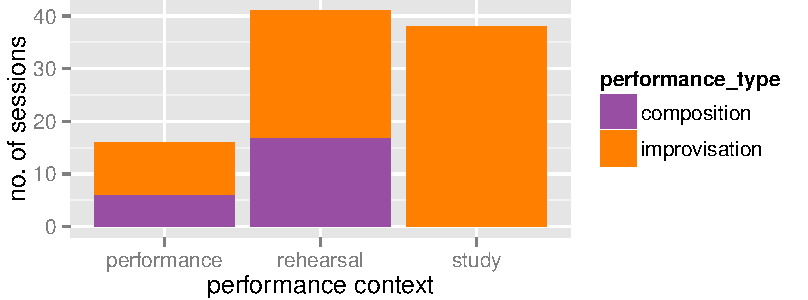
\includegraphics[width=\linewidth]{figures/sessions-count}
  \caption{Distribution of the sessions in our interaction corpus by
    performance context. Improvisations or compositions were repeated
    several times in rehearsals and study sessions but only performed
    once in concerts.
    \label{fig:count-data}}
\end{figure}


\subsection{Differentiating interaction sessions}
\label{differentiating-interaction-sessions}

\begin{figure} \centering
  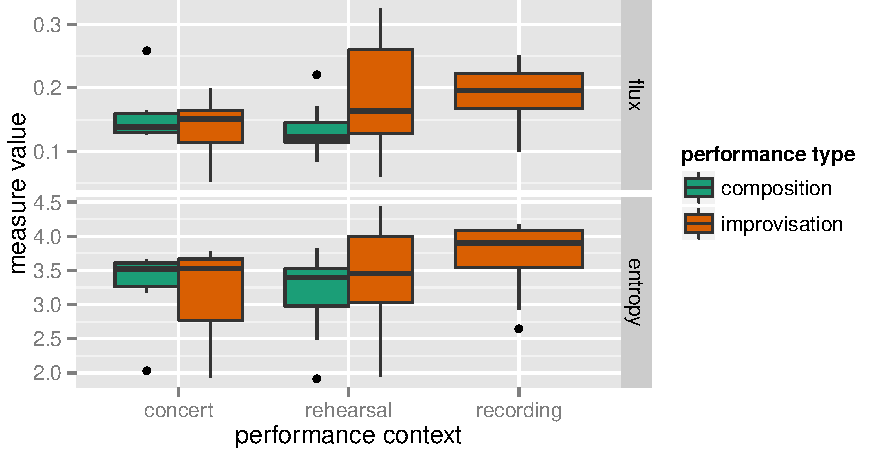
\includegraphics[width=\linewidth]{figures/context-flux-entropy-boxplot}
  \caption{Distributions of flux and entropy values by performance
context. Study and rehearsal sessions had the highest flux for
improvisations. Compositions had lower
flux in rehearsals than performances.
\label{fig:flux-entropy-boxplot}}
\end{figure}

The distribution of flux and entropy with respect to session contexts,
types and instrumentation are shown in Figure
\ref{fig:flux-entropy-boxplot}. A three-way ANOVA procedure was
performed on the data set to find whether the metatdata could
significantly predict the entropy and flux values.
% TODO we haven't explained what ``the 95 performative sessions'' are,
% have we?
In the following analysis, only the 95~``performance context''
sessions were considered, excluding the demonstration and
data-collection contexts. TODO can we justify this?

All main effects on flux were found to be significant: performance
context ($F(2,86) = 6.28, p < 0.01$), performance type
($F(1,86) = 7.21, p < 0.01$), and instrumentation
($F(1,86) = 20.06, p < 0.001$). Significant interaction effects were
also found for performance context and type
($F(1,86) = 6.18, p < 0.05$), and performance context and
instrumentation ($F(1,86) = 10.48, p < 0.01$).

For entropy, significant main effects were found due to performance
context ($F(2,86) = 12.10, p < 0.001$), and instrumentation
($F(1,86) = 25.86$). The interaction of performance type and
instrumentation was also found to be significant
($F(1,86) = 9.93, p<0.01$).

These tests show that the different interaction styles that might be
present in performance contexts, types and instrumentations are
reflected in the values of flux and entropy of their transition
matrices.

\begin{figure*}[t!]
    \centering
    \begin{subfigure}[t]{0.5\linewidth}
        \centering
          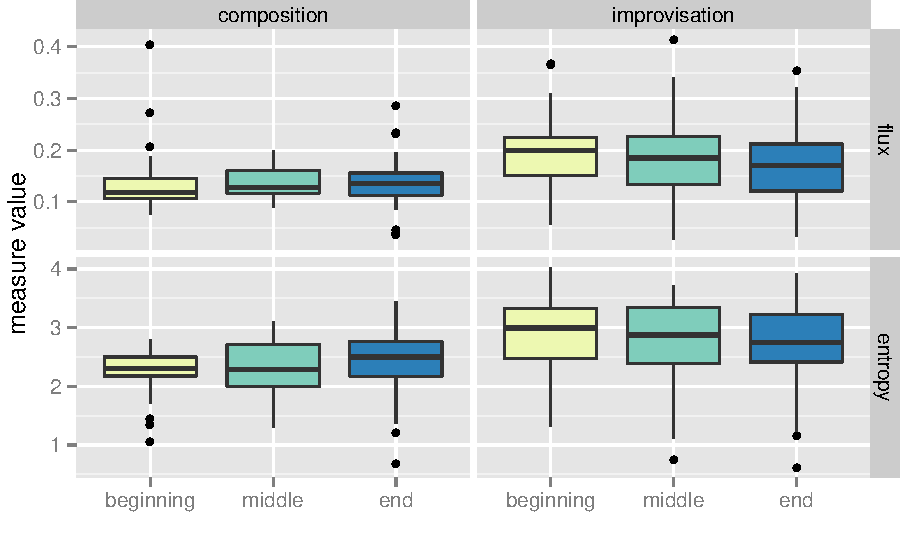
\includegraphics[width=\linewidth]{figures/type-section-flux-entropy}
          \caption{Performances divided by performance type. \label{fig:type-section-flux-entropy}}
    \end{subfigure}%
    ~ 
    \begin{subfigure}[t]{0.5\linewidth}
        \centering
          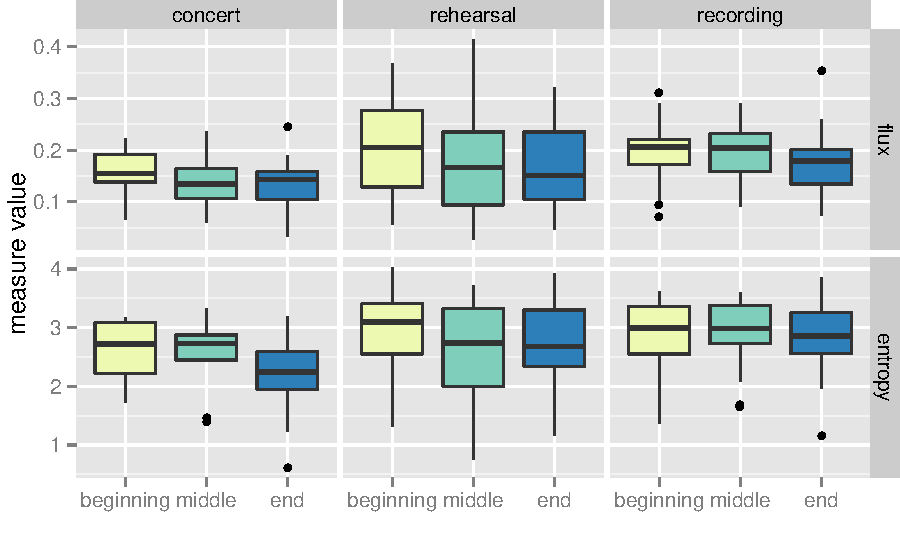
\includegraphics[width=\linewidth]{figures/context-section-flux-entropy}
          \caption{Sessions divided by performance context. \label{fig:context-section-flux-entropy}}
    \end{subfigure}
    \caption{The flux and entropy of different interaction sessions
      divided into beginning, middle, and end.}
\end{figure*}


\subsection{Breaking performances into sections}

It is clear from these results that flux and entropy can be used to
differentiate between performance styles and types, but can they be
used to understand some of the internal structure of performances? A
simple model for understanding temporal art-forms is the ``beginning,
middle, end'' structure. To investigate how this structure fits our
corpus, we can divide the gestural-sequences of each session into
thirds and calculate the transition matrices given by each section.

Figure~\ref{fig:type-section-flux-entropy} shows that the flux and
entropy of compositions are much more stable with respect to section
than for improvisations. The stability of compositions is to be
expected since performers are expected to use the same gestures in
each rehearsal and performance of a composition, it may be that
different kinds of compositions could result in different structural
differences. Both measures have a downward trend through sections in
improvisations with Kruskal-Wallis tests showing a significant effect
of section on flux ($\chi^2(2)=5.8, p=0.05$). This could be explained
by performers entering an exploration stage at the start of an
improvisation, where they change gesture frequently to experiment with
different ideas. At the end of an improvisation, performers may change
gesture less frequently while ``winding up'' the performance.

The gestural change in improvisation can be further explored by
dividing the sessions by performance context. Figure
\ref{fig:context-section-flux-entropy} shows this division for
improvisations only. In rehearsals and studies the distribution of
flux and entropy over sections has a similar shape, both measures drop
in the ending section of studies and after the beginning section in
rehearsals. In performances however, flux drops after the beginning
while entropy drops substantially in the ending section. This
indicates a more constrained performance style in this closing
section, where performers transition between fewer gestures in the
final section of performances.

% todo add the plots here.

% \begin{figure}
%   \centering
%   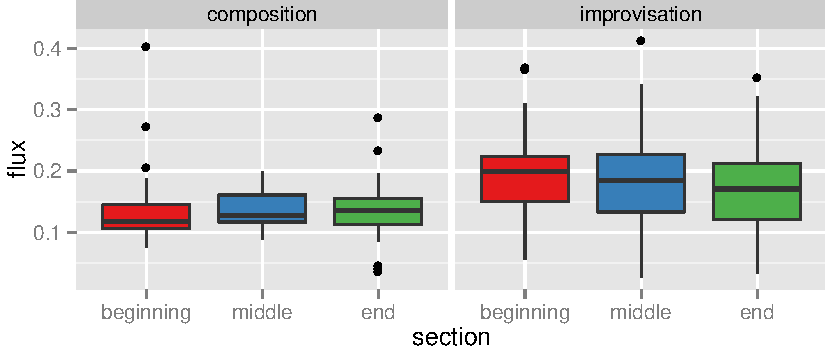
\includegraphics[width=\linewidth]{figures/type-section-flux}
%   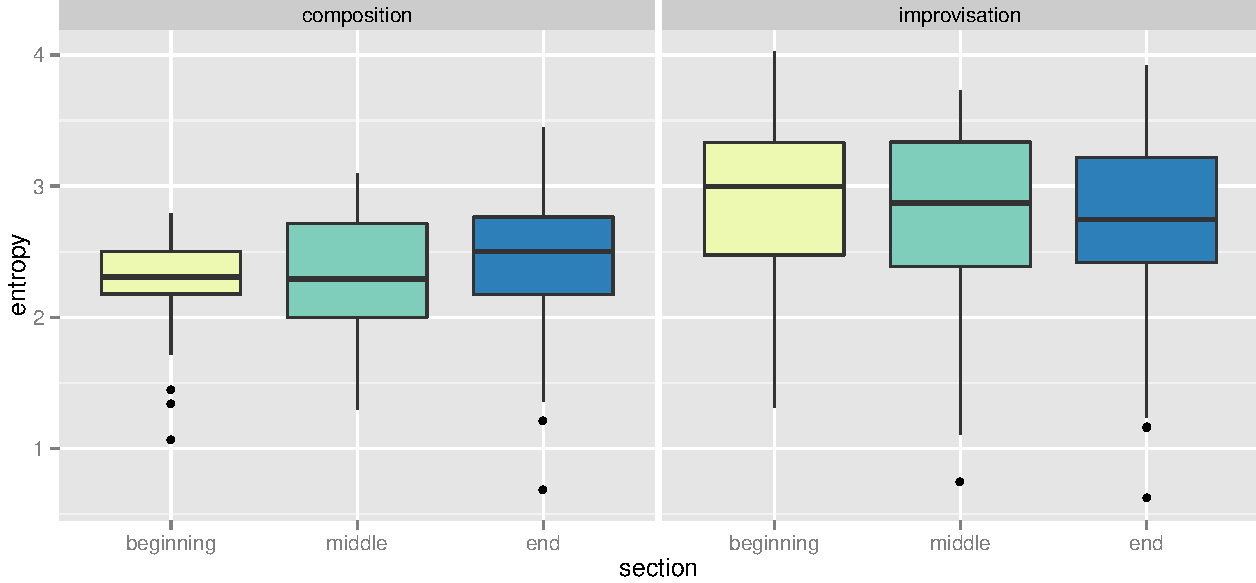
\includegraphics[width=\linewidth]{figures/type-section-entropy}
%   \caption{The flux of compositions and improvisations divided into
%     beginning, middle, and end. Composition flux remains stable throughout,
%     but improvisations show a downward trend and composition entropy tends to move up
%     at the end, while flux moves down.
%     \label{fig:type-section-flux-entropy}}
% \end{figure}

% \begin{figure}
%   \centering
%   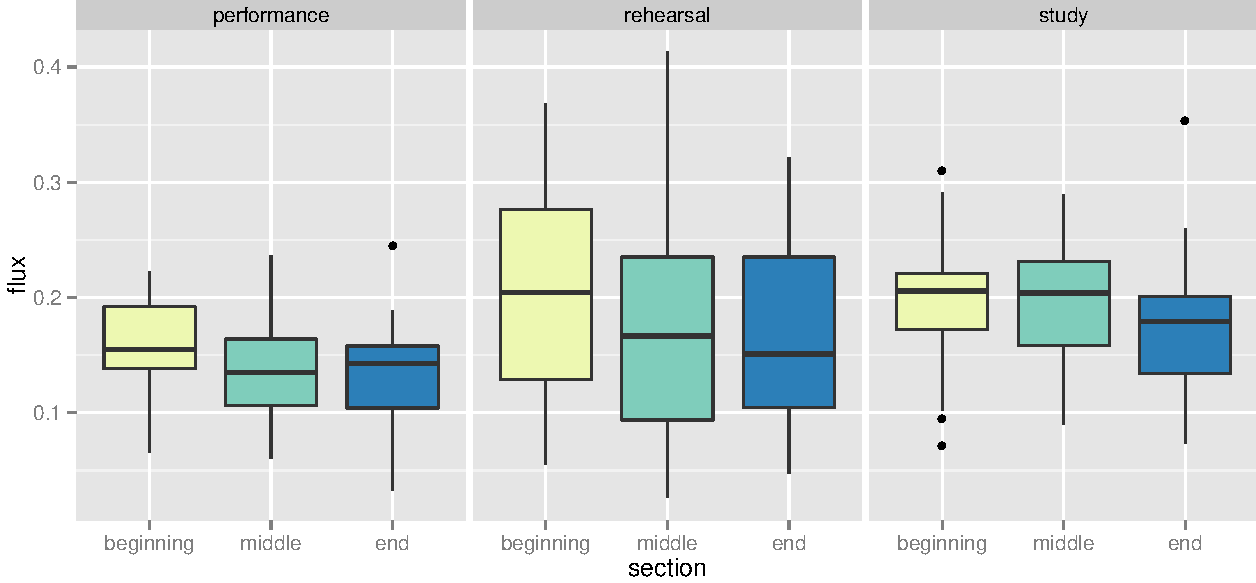
\includegraphics[width=\linewidth]{figures/context-section-flux}
%   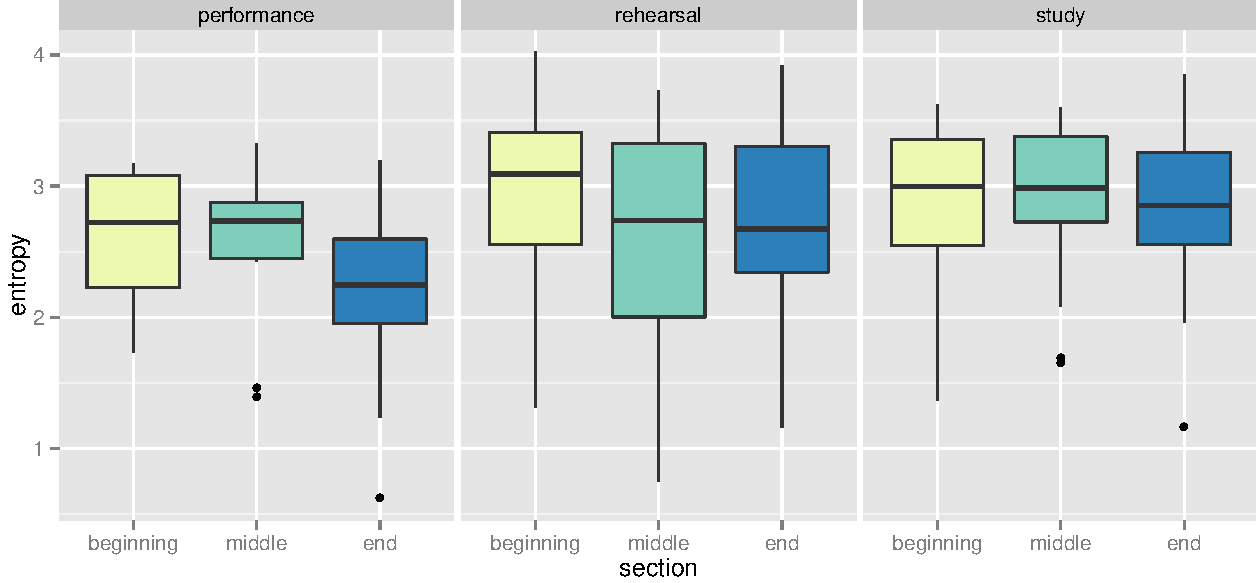
\includegraphics[width=\linewidth]{figures/context-section-entropy}
%   \caption{The distribution of flux and entropy in performances divided by ``beginnings,
%     middles, and ends''.
%     \label{fig:context-section-flux-entropy}}
% \end{figure}

\subsection{Performance styles over time}

While the interaction session in our corpus have many different
contexts, they are all part of a program of artistic and HCI research
that has evolved over time. Figure \ref{fig:flux-entropy-through-time}
shows the values of flux and entropy for each session in the corpus.
Over the course of this research program, different ensembles and
different activities have been emphasised, some of these differences
can be seen as clusters of performances with similar flux and entropy
in the two plots. For instance, the earliest series of rehearsals and
performances had flux between 0.05 and 0.15, while the period of
activity after July 2014 had flux between 0.1 and 0.25. This change
corresponded with an intensive series of study sessions and rehearsals
where the participants developed a more ``fluctuating'' style of
performance. The entropy between these two periods, however, remains
at a similar level, showing the the space of available gestures that
the performers explored was relatively stable.

\begin{figure}
  \centering
  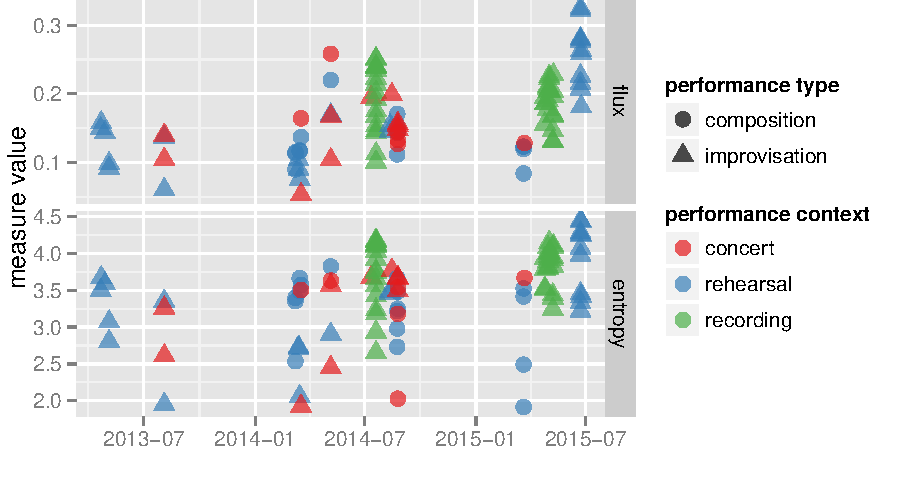
\includegraphics[width=\linewidth]{figures/flux-entropy-through-time}
  \caption{Distribution of flux and entropy values of sessions through time.
    Different performance styles are visible as clusters of similar
    flux regardless of performance context.
    \label{fig:flux-entropy-through-time}}
\end{figure}

\section{Conclusions}

In this paper we have extended our previous work on transition
matrices with two simple matrix measures, flux and entropy, both of
which have been demonstrated to have significant discriminatory power
with regards to a corpus of 150 collaborative touch-screen
interactions. Not only do these measures differentiate between
different types of sessions and the internal structure of these
sessions, but they have explanatory power that has thrown new light on
the musical interactions under examination. HCI researchers are
increasingly concerned with interactions that happen in-the-wild,
where the interactions of many users may be collected without the
opportunity to survey or interview users. We suggest that analysing
interaction-state transitions using matrices and simple measures can
lead to new insights into HCI interactions outside the lab. 


%TODO Mention Manovich transmutation stuff
The macro-gestures that these processes reveal could also be used as
the basis for new works of new media art~\cite{Manovich:2002ly}.

%\pagebreak
\bibliographystyle{SIGCHI-Reference-Format}
\bibliography{references}

\end{document}

%%% Local Variables:
%%% mode: latex
%%% TeX-master: t
%%% End:
